\section{Implementation \& Verification}\label{sec:implementation_and_verfication}

In this section the suggested structure in section \ref{sec:Structure}, implemented with the numerical solutions in section \ref{se:preissmann_scheme}-\ref{sec:concentrate}, is tested and verified.

The first part to be elaborated upon is the initialization.

 \subsection*{Initialization}

For the setup procedure of the simulation in list form, the specifications part shown in figure \ref{fig:sys_setup} needs to be defined. The parameters in the list for both pipe and tank can be seen in table \ref {tab:init_list}. 

\begin{enumerate} \label{tab:init_list}
	\item Pipe
	\begin{itemize}
		\item Length [m]
		\item Sections (Number of sections the pipe should be split in to)
		\item $\text{I}_\text{b}$ (Slope) [\textperthousand]
		\item $\Delta$x = Length/Sections [m]
		\item Diameter [meter]
		\item Theta (parameter used in Preissmann scheme)
		\item $\text{Q}_{\text{f}}$ (maximum flow found by Manning formula, see equation \ref{eq:qf_for_flow}) [$\text{m}^\text{3}/\text{s}$]
		\item Side/lateral inflow present 
		\item Section location in data 
	\end{itemize}
	\item Tank
	\begin{itemize}
		\item Size [$\text{m}^\text{3}$]
		\item Height [m]
		\item Area = Size / Height [$\text{m}^\text{2}$]
		\item Maximum outflow [$\text{m}^\text{3}/\text{s}$]
		\item Section location in data 
	\end{itemize}
	%b\caption{Table of needed parameters for pipe and tank}
\end{enumerate}

Some parameters can be found from others and is set to be calculated automatically. Furthermore an item is added that indicates in which section of the obtained simulation data the specific output of the component is located. This item is given the number of the order in which the component appears in the list. To give an overview of the system to be simulated, and to easily be able to locate specific parameters needed during simulation, three structures is returned to the workspace. These are named ``pipe\_spec'', ``tank\_spec'' and ``sys\_setup''. The first two structures holds the information shown in table \ref{tab:init_list} respectively. The last one, ``sys\_setup'', holds information of the various parts indexed in the order the system is setup and simulated. In figure \ref{fig:sys_setup_matlab} the content of ``sys\_setup'' is shown for a setup with two pipes and a tank.

\begin{figure}[H]
\centering
\includegraphics[width=0.5 \textwidth]{report/simulation/pictures/sys_setup_matlab.png}
\caption{Display of structure holding system setup information in MATLAB.}
\label{fig:sys_setup_matlab}
\end{figure}

An initialization scheme is constructed as per figure \ref{fig:simple_sewer} where adjoint pipes is considered as one part of the system and tank is used as a separator between parts.
The iterative scheme shown in figure \ref{fig:preissmann_grid_scheme_exampel} requires that boundary conditions is found before the iterative Preissmann scheme can be started. It has been decided by the project group that input should be given in flow, as input in height would be needed to be specific for the pipe inserted, to make the simulation universal. This means that from an initial input flow the corresponding height in the pipes needs to be found. By equation \ref{eq:calc_for_flowv2} flow can be obtained from height, but the equation is transcendental i.e. can not be solved analytically for height. This means that other means is necessary to obtain height from flow. This can be done in several ways, but the initial solution chosen is to use the MATLAB curve fitting toolbox.
For each pipe, during initialization, a data set from zero to the diameter of the pipe in thousand steps is created, and from which the corresponding flow is obtained by equation \ref{eq:calc_for_flowv2}.

\begin{figure}[H]
 \centering
 % This file was created by matlab2tikz.
%
%The latest updates can be retrieved from
%  http://www.mathworks.com/matlabcentral/fileexchange/22022-matlab2tikz-matlab2tikz
%where you can also make suggestions and rate matlab2tikz.
%
\definecolor{mycolor1}{rgb}{0.00000,0.44700,0.74100}%
%
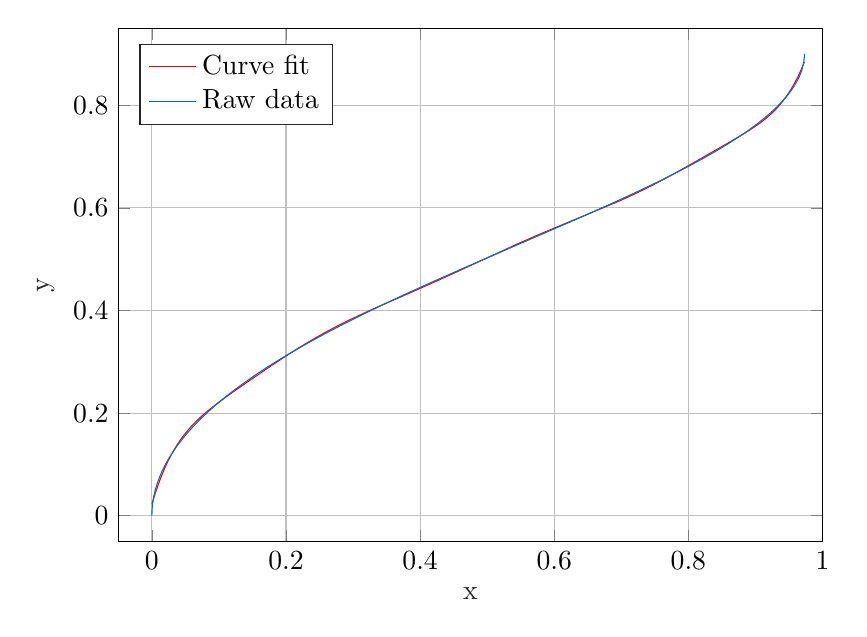
\begin{tikzpicture}

\begin{axis}[%
width=3.521in,
height=2.566in,
at={(0.758in,0.481in)},
scale only axis,
xmin=-0.05,
xmax=1,
xlabel style={font=\color{white!15!black}},
xlabel={x},
ymin=-0.05,
ymax=0.95,
ylabel style={font=\color{white!15!black}},
ylabel={y},
axis background/.style={fill=white},
xmajorgrids,
ymajorgrids,
legend style={at={(0.03,0.97)}, anchor=north west, legend cell align=left, align=left, draw=white!15!black}
]
\addplot [color=red]
  table[row sep=crcr]{%
0	0.0222641876397454\\
0.00583788013141662	0.0468505124572859\\
0.0116757602628333	0.0685037472280541\\
0.01751364039425	0.0875962984430564\\
0.0233515205256666	0.104462594043742\\
0.0291894006570832	0.119402060847026\\
0.0350272807884998	0.132681928352076\\
0.0408651609199165	0.14453986606579\\
0.0467030410513332	0.155186461298207\\
0.0535139012046525	0.166323129330026\\
0.0603247613579719	0.176319581381477\\
0.0681086015331941	0.186627394570619\\
0.0768654217303191	0.1971234679247\\
0.0865952219493469	0.207784706738995\\
0.0982709822121801	0.219634930070442\\
0.113838662562624	0.23449066785112\\
0.138163163110194	0.256755738358134\\
0.176109383964402	0.290671244351543\\
0.201406864533874	0.312526360051635\\
0.221839444993832	0.329374050052282\\
0.240326065409985	0.34381856012056\\
0.257839705804235	0.35673446219757\\
0.275353346198485	0.368905237211488\\
0.293839966614638	0.381009693497422\\
0.314272547074596	0.393647570538794\\
0.339570027644068	0.408528726872221\\
0.390164988783012	0.437347221406009\\
0.429084189659123	0.459928516339826\\
0.468003390535234	0.483262809711989\\
0.54389583224365	0.528968698128539\\
0.574058212922636	0.546263994393304\\
0.604220593601622	0.562860267064146\\
0.696653695682386	0.613119065583713\\
0.717086276142344	0.62530025086964\\
0.736545876580399	0.637586486102553\\
0.756005477018455	0.650574852430809\\
0.777411037500316	0.665605335087019\\
0.803681498091691	0.684833203666043\\
0.864979239471565	0.730734878672607\\
0.884438839909621	0.745858014555948\\
0.897087580194357	0.756440925031475\\
0.906817380413385	0.765353228191959\\
0.914601220588607	0.773208230042211\\
0.922385060763829	0.781942336734848\\
0.929195920917148	0.790515086732738\\
0.935033801048565	0.798722858348917\\
0.940871681179982	0.807888165233192\\
0.946709561311398	0.818188953039921\\
0.952547441442815	0.829827057099856\\
0.958385321574232	0.8430304635012\\
0.963250221683745	0.855413188684596\\
0.968115121793259	0.869225396536382\\
0.972980021902773	0.884648045759077\\
};
\addlegendentry{Curve fit}

\addplot [color=mycolor1]
  table[row sep=crcr]{%
0	0\\
0.00030642296001504	0.01233\\
0.00122592449248948	0.02466\\
0.00275919619829157	0.03699\\
0.00492531381189298	0.04941\\
0.00771691837291222	0.0618300000000001\\
0.0111359602571995	0.07425\\
0.0152163500161991	0.0867600000000001\\
0.0199744759873318	0.09936\\
0.02542711466865	0.11205\\
0.0315913434853029	0.12483\\
0.0384338333138317	0.13761\\
0.0460682367603654	0.15057\\
0.0544660114484651	0.16362\\
0.0637094855914684	0.17685\\
0.0738302832003164	0.19026\\
0.0847840346449592	0.20376\\
0.0967472281174419	0.21753\\
0.109678802055319	0.23148\\
0.123697951078652	0.2457\\
0.138846482140551	0.26019\\
0.155163670747372	0.27495\\
0.172793050923732	0.29007\\
0.191782482726017	0.30555\\
0.212292745916907	0.32148\\
0.234499027859045	0.33795\\
0.25845887409398	0.35496\\
0.284486130286045	0.37269\\
0.312918691318617	0.39132\\
0.344254168236911	0.41112\\
0.37915911064623	0.43245\\
0.419079139891965	0.45612\\
0.466907719593891	0.48375\\
0.53413117460992	0.52182\\
0.638838688603708	0.58113\\
0.684244287950606	0.60759\\
0.720760960442891	0.62955\\
0.751794914662872	0.6489\\
0.778966712722586	0.66654\\
0.802970121524758	0.68283\\
0.824328787062596	0.69804\\
0.843524532554507	0.71244\\
0.860764663768599	0.72612\\
0.87624717181071	0.73917\\
0.890156294853092	0.75168\\
0.902569357193314	0.76365\\
0.913654569164784	0.77517\\
0.923559217305502	0.78633\\
0.93233869141443	0.79713\\
0.94005219868443	0.80757\\
0.946818481487701	0.81774\\
0.952682361805689	0.82764\\
0.957734233356883	0.83736\\
0.962003234496279	0.8469\\
0.9655201136824	0.85626\\
0.968316966985129	0.86544\\
0.97044491415244	0.87453\\
0.971919271555091	0.88353\\
0.972756442059394	0.89244\\
0.972980021902773	0.9\\
};
\addlegendentry{Raw data}

\end{axis}
\end{tikzpicture}%
\caption{Comparison between data curve fitted to a ninth order polynomial and raw data.}
\label{fig:curvefit_comparision}
\end{figure}
